\chapter{Rationale}\label{chap:rationale}

\section{Introduction}

The research project, titled "Overall Power Optimization of Thread Mesh Wireless Network," is a child project within the broader MOOD-Sense initiative. The MOOD-Sense project employs IoT devices to detect and predict challenging behavior in dementia patients. The project aims to develop an early warning system combining sensors, artificial intelligence, and wireless communication to provide feedback for healthcare professionals and improve patient care and safety \cite{MOOD-Sense_Research}. To further enhance the connectivity and scalability among IoT devices in the MOOD-Sense project, a new network protocol called Thread is proposed to be implemented. Thread is a low-power, IPv6-based, mesh networking protocol specifically designed for IoT applications, offering secure, reliable, and efficient communication. It supports self-healing networks with robust routing capabilities and features like end-to-end encryption, making it an ideal choice for the MOOD-Sense initiative \cite{Thread_Group_Benefits}.

The primary focus of this child project is to optimize the energy efficiency of the wireless Thread network protocol utilized by different wireless sensors and various MOOD-Sense projects. To achieve this, the project examines transmission power network parameter and configuration such as device types, path loss, positions, and RSSI with the objective of determining their optimal configuration.

In order to optimize the transmission power network parameter and reduce overall power consumption, the child project establishes a Thread network and employs an algorithmic approach using appropriate hardware. The ultimate goal is to investigate the impact of transmission power parameter optimization on maintaining reliable communication between devices while minimizing power consumption.


\section{Present Situation}\label{sec:present_situation}
The MOOD-Sense research project originally planned to use three wireless communication technologies: BLE, ZigBee, and Wi-Fi for network communication. However, without a central network protocol, various subprojects within MOOD-Sense, such as dementia patient behavior registration and environmental context monitoring, are being carried out separately. This separation leads to disconnected devices and makes data sharing and integration difficult. The current situation can be visualized as a diagram, showing isolated subprojects and devices without an integrated network.

\begin{figure}[H]
    \centering
    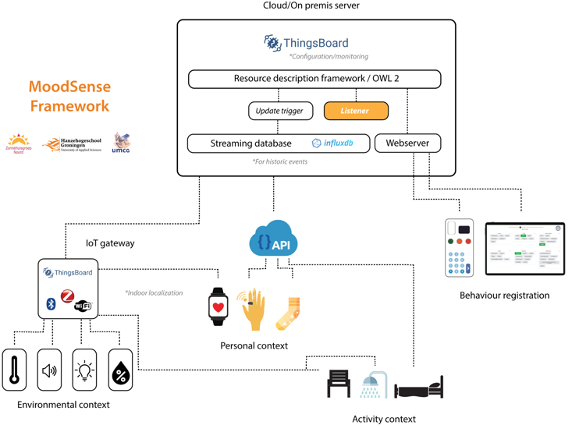
\includegraphics[width=0.8\textwidth]{images/rationale/rationale_present_situation.png}
    \caption{Current state of the MOOD-Sense initiative.}
    \label{fig:rationale_present_situation}
\end{figure}

To address these challenges and create an energy-efficient network, the proposal to implement a Thread mesh wireless network was introduced. Thread's features, such as mesh networking, multiprotocol support, and low cost, make it an ideal solution for connecting BLE, ZigBee, and Wi-Fi connectivity together. By adopting the Thread mesh network protocol, seamless connectivity, interoperability, and communication among all devices within the MOOD-Sense framework can be achieved. This implementation paves the way for the desired outcome of an optimized, low-power, and reliable network.


\section{Desired Outcome}\label{sec:desired_outcome}
The desired outcome of this research is to develop an efficient algorithm that integrates seamlessly within the Thread-based wireless network system and optimizing power consumption. This algorithm will not only adjust transmission power but also select the most suitable device types for the network, contributing to energy efficiency and reliable communication. A schematic overview of the system with the integrated algorithm is as follows:

\begin{enumerate}
    \item \textbf{Input}: The primary input parameters for the network optimization algorithm include the total number of devices and the distance between each device. These inputs provide the necessary data to guide the optimization process and ensure that the algorithm makes informed decisions regarding device types and transmission power levels.
    \item \textbf{Algorithm}: The power optimization algorithm consists of two stages: the Monte Carlo Method and the Genetic Algorithm. In the first stage, MCM focuses on determining the right device types based on various constraints and constructing an optimal network configuration with an initial transmission power setting. The second stage involves GA, which takes the output from MCM and optimizes the transmission power settings to minimize power consumption while maintaining network reliability.
    \item \textbf{Integration}: The algorithm will run separately on a dedicated system and generate output for optimal device types and transmission power settings. This output will then be manually integrated into the Thread devices, ensuring that the devices are configured for optimal performance based on the algorithm's recommendations.
    \item \textbf{Optimization}: In the optimization process, the MCM algorithm initially finds the right device types and builds the optimal network configuration with the initial transmission power, considering various constraints. Afterward, the GA algorithm takes this output and optimizes the transmission power settings to make the network as low-powered and energy-efficient as possible, without compromising on reliability.
    \item \textbf{Output}: The output consists of the appropriate device types for a reliable Thread network configuration, along with the optimal transmission power settings for each device. This output enables the creation of an energy-efficient and reliable Thread-based wireless network that meets the needs of the MOOD-Sense initiative and other similar IoT applications.
\end{enumerate}

By achieving this desired outcome, the algorithm will provide a comprehensive solution for power optimization in Thread networks, supporting the MOOD-Sense initiative and similar IoT applications in building energy-efficient and sustainable networks.


\section{Problem Definition}\label{sec:problem_definition}
As the adoption of IoT devices in applications like the MOOD-Sense initiative increases, there is a growing need for energy-efficient and reliable wireless network protocols. The Thread network protocol offers low-power and reliable mesh networking, making it suitable for such applications. However, optimizing power consumption while maintaining network reliability remains a challenge. Additionally, the selection of appropriate device types is crucial for building an efficient Thread network, as Thread offers various device types depending on the use case.

The primary goal of this research is to determine the most effective algorithmic approach for power optimization in a Thread-based wireless network, specifically through transmission power adjustments and the selection of the right device types. By focusing on these aspects, the research will contribute to the development of energy-efficient network solutions for the MOOD-Sense initiative and similar IoT applications. This approach ensures the proper selection and utilization of devices within the Thread network, optimizing the overall network performance and energy efficiency.


\section{Research Questions}\label{sec:research_questions}

\subsection*{Main Research Question}
How can parameter optimization be applied to develop a power-optimized Thread mesh wireless network?


\subsection*{Sub-Research Questions}
\begin{enumerate}
    \item What are the key features of the Thread protocol that make it suitable for IoT applications, specifically in the context of the MOOD-Sense project?
    \item Which parameters significantly impact the transmission power in a Thread network, and how do they relate to energy efficiency and network performance?
    \item How do the Monte Carlo Method (MCM) and the Genetic Algorithm (GA) differ in their approach to optimizing transmission power in a Thread network, and what are the key steps for their implementation?
    \item What are the specific hardware requirements for implementing a Thread network, and how do they influence the network's energy efficiency and performance in the context of power optimization?
    \item How do variations in algorithmic parameters impact the performance of MCM and GA in optimizing wireless network transmission power and path loss?
    \item Are there any differences in power optimization performance between different iterations for both Maximum and Optimized modes?
    \item How do the different devices perform in terms of power optimization when comparing the Maximum and Optimized modes?
    \item Is there a correlation between mean, max, and min current values and the efficiency of power optimization for both Maximum and Optimized modes?
    \item How does the location impact the power optimization performance of the Maximum and Optimized modes?
    \item How does the performance of the MCM and GA modes differ across different device types, and what impact does this have on current consumption?
    \item How do MCM and GA modes compare with Maximum mode in terms of efficiency across various locations and device types?
    \item What is the significance of errors in the power optimization process and their impact on the performance of MCM and GA modes?
\end{enumerate}


\section{List of Requirements}\label{sec:list_of_requirements}
Focusing on power optimization in the Thread mesh wireless network protocol and ensuring reliable communication, the following requirements address the challenges related to power consumption and sustainability in Thread mesh wireless networks and guide the research process:

\begin{enumerate}
    \item Optimize power efficiency for the Thread network protocol with a focus on minimizing power consumption while maintaining reliable communication.\\
    \textbf{Constraint}: The optimization should not compromise the network's stability or communication quality.
    \item Apply Monte Carlo and Genetic Algorithm for optimizing transmission power and determining efficient network configurations.\\
    \textbf{Constraint}: The optimization techniques should be computationally feasible and should not add significant overhead to the network's operation.
    \item Develop a power-optimized Thread mesh wireless network by considering the optimal device types for different nodes.\\
    \textbf{Constraint}: The selected device types should maintain low power consumption while meeting the network's performance requirements.
    \item Assess the impact of location on power optimization performance for both Maximum and Optimized modes.\\
    \textbf{Constraint}: The assessment should consider diverse environments to ensure the results are applicable to various real-world situations.
    \item Compare the performance of MCM and GA modes across different device types and locations in terms of power optimization.\\
    \textbf{Constraint}: The comparison should be fair and unbiased, taking into account the specific characteristics of each device type and optimization technique.
    \item the significance of errors in the power optimization process and their impact on the performance of MCM and GA modes.\\
    \textbf{Constraint}: The investigation should identify potential sources of errors and recommend ways to minimize their impact on power optimization performance.
    \item Suggest future research directions and improvements for Thread network optimization, including device positioning, path loss, and broader application scope.\\
    \textbf{Constraint}: The suggestions should be realistic and feasible, considering existing limitations and challenges in the field.
    \item Ensure the research adheres to responsible research and innovation principles, including ethical aspects, professional skills, applied research, and sustainability.\\
    \textbf{Constraint}: The research should prioritize the development of sustainable solutions and maintain transparency and accountability throughout the process.
\end{enumerate}
